\documentclass[11pt]{article}
\usepackage[utf8x]{inputenc}
\usepackage[T1]{fontenc}
\usepackage{graphicx}
\usepackage{grffile}
\usepackage{longtable}
\usepackage{wrapfig}
\usepackage{rotating}
\usepackage[normalem]{ulem}
\usepackage{amsmath}
\usepackage{textcomp}
\usepackage{amssymb}
\usepackage{capt-of}
\usepackage{hyperref}
\usepackage{svg}
\usepackage[margin=1.0in]{geometry}
\author{Brett Viren}
\date{\today}
\title{Wire-Cell Toolkit Imaging}
\hypersetup{
 pdfauthor={Brett Viren},
 pdftitle={Wire-Cell Toolkit Imaging},
 pdfkeywords={},
 pdfsubject={},
 pdfcreator={Emacs 26.1 (Org mode 9.1.14)}, 
 pdflang={English}}
\begin{document}

\maketitle

\section{Introduction and Scope}

This (very informal and sloppy) note documents the Wire-Cell Toolkit (WCT) ionization electron distribution reconstruction package \texttt{wire-cell-img} aka \textit{3D imaging}. 
It describes the algorithms and their implementation. 
First it describes basic building blocks of \textit{rays} and how they are used to define coordinate systems called \textit{ray grids} which allow fast queries on the wire geometry. 
These ray grids are then used to implement the core algorithm, from which first Wire-Cell derived its name, termed \textit{tiling}. 
This restricts regions of a 2D plane in each readout time slice across channels which may contain ionization electrons. 
Then a channel \textbf{grouping} is performed to reduce the size of the problem of the final step called \textit{solving}.

\section{Rays Basics}
\label{sec:raybasics}

In WCT, in the \texttt{WireCell} namespace, a \texttt{Ray} is simply a \texttt{std::pair<Point,Point>} defined in \texttt{wire-cell-util} in the \texttt{Point.h} header.  Conceptually it represents an relative vector pointing from \texttt{Ray::first} and to \texttt{Ray::second}.  Various vector operations are defined on \texttt{Point} and \texttt{Ray}.  Note, one may see \texttt{Vector} used.  It is a synonym for \texttt{Point} and sometimes used to semantically distinguish between a relative displacement and an absolute point. 

Rays may be used in several contexts and one critical one is in describing geometry related to wires (as always, this means wire segments).  The rest of this section describes how rays are used to implement the core Wire-Cell imaging algorithms.  It covers a progression of functionality:

\begin{description}
\item[grid] construction of a set of grids defined in terms of rays which allow fast \emph{addressing} of special points in a 2D space
\item[tiling] partitioning the 2D space, based on the grid, to constrain location of activity
\item[clustering] combining elements of the 2D tiling along a third dimension
\item[grouping] combining overllaping ``sources'' (``blobs'') and ``measurements'' (``merged channels'') 
\item[solving] determine the amount of ionization activity likely in a regions localized by tiling. 
\end{description}

This functionality is based on bounding regions of the 2D plane with pairs of parallel rays.  A region is considered to have infinite extent along the mutual direction of its bounding rays and to have finite extent along the perpendicular direction.  This finite extent is represented by a \textbf{pitch} vector which has its end points on both rays.  The ray on the tail of the pitch vector is considered inside the region while the other ray is considered outside.   That is, the region is half-inclusive.  


\section{Ray Grid}
\label{sec:raygrid}

The wire segments in a pair wire planes provide a basis for a non-orthogonal grid.  Under the assumption that the wires share a common pitch and angle the grid is uniform.  This assumption allows for optimization in calculating crossing ray crossing points in terms of indexed grid points.  It further allows optimization in calculating the location of a crossing point in terms of the pitch location of a third plane.  

A generalized \emph{ray grid} as consisting of a number of coplanar \emph{layers}.  Each layer is composed of a infinite number of parallel rays of uniform pitch which may be generated by specifying an ordered pair of two neighboring rays.  The \emph{pitch vector} of this layer is generated as running perpendicular to both rays and of magnitude that of their separation.  A three-layer ray grid is illustrated in figure \ref{fig:raygrid}.

\begin{figure}[htbp]
\centering
\includesvg[width=1.0\textwidth]{figs/test_raytiling-00}
\caption{\label{fig:raygrid}
The points and vectors involved in constructing and using ray grids.}
\end{figure}


A number of vectors are defined.  Their superscript indices label a layer and their subscripts label grid indices.

\begin{description}
\item[{\(p^l\)}] the pitch vector for layer \(l\)
\item[{\(c^n\)}] a special center point on \emph{ray 0} of layer \(n\)
\item[{\(r^{lm}_{ij}\)}] the crossing point of ray \(i\) from layer \(l\) and ray \(j\) from layer \(m\)
\item[{\(r^{lm}_{00}\)}] the crossing point the zero rays of layers \(l\) and \(m\).
\item[{\(w^{lm}\)}] a vector giving the displacement along the direction of a ray in layer \(l\) between the crossing points of that ray and two neighboring rays from layer \(m\)
\end{description}

This last two tensors, \(r^{lm}_{00}\) and \(w^{lm}\) can be calculated with simple vector arithmetic (see \texttt{ray\_pitch()} from \texttt{Point.h}), pair-wise among the \(N_l\) layers in the ray grid.  The former is symmetric and both have undefined diagonals and so require \(\mathcal{O}(N_l^2)\) operations where \(N_l\) is the number of layers (typically \(N_l = 5\) as described below).  Given these two tensors, arbitrary crossing points of rays from different layers can be written as

\begin{equation}
r^{lm}_{ij} = r^{lm}_{00} + j w^{lm} + i w^{ml}
\end{equation}

which provides a faster calculation than the vector arithmetic required to find the crossing points of arbitrary rays.  

Locating crossing points of rays from two layers in a third layer is another fundamental operation.  Given that these crossing points are on the ray grid a tensor equation can be written:

\begin{equation}
p^{lmn}_{ij} = (r^{lm}_{ij} - c^n) \cdot \hat{p}^n
\end{equation}
Expanding \(r^{lm}_{ij}\), 

\begin{equation}
P^{lmn}_{ij} = r^{lm}_{00}\cdot \hat{p}^n + jw^{lm} \cdot \hat{p}^n + iw^{ml} \cdot \hat{p}^n - c^n \cdot \hat{p}^n
\end{equation}

Given the tensor symmetries, one can express more simply this as: \(P^{lmn}_{ij} = ja^{lmn} + ia^{mln} + b^{lmn}\).  The tensors \(a\) and \(b\) are scalar valued, \(a\) is not symmetric under a transpose of \(l\) and \(m\) and \(b\) is.  Both have undefined diagonals.  That is, \(l, m, n\) must be mutually unique.  Finally, it is common to look up some quantity that is indexed by the ray index.  This can be found simply a \(I^{lmn}_{ij} = floor(P^{lmn}_{ij}/p^n)\).

\section{Ray Tiling}
\label{sec:raytiling}

Central to Wire-Cell 3D imaging is the concept of ``tiling''.  This is a partitioning of the 2D plane that is transverse to the electron drift direction by considering the measured signal samples from all channels summed over some slice of time (typically a few ms).  The partitioning is performed along lines which are parallel to the wires of the planes on one face of an anode.

The goal of the tiling is to identify regions where ionized electrons likely existed in the time slice.  The procedure involves selecting all wires attached to all channels which collected signal (after response deconvolution) above some threshold.  These are called \emph{active wires}.  The ray parallel to an active wire and residing half way along the negative pitch direction to the active wires nearest neighbor is called an \emph{active ray}.  That is, an active ray provides the lower bounds of an  \emph{active strip} which is one pitch wide and centered along the active wire.

This is illustrated in figure \ref{fig:activity}.  It represents a simple simulation of a time slice.   Clumps of points are generated and for each point the nearest wire from each layer is located and its activity count is incremented.  


\begin{figure}[htbp]
\centering
\includesvg[width=1.0\textwidth]{figs/test_raytiling-01}
\caption{\label{fig:activity}
Depiction of the location of generated ``electrons'' in a toy simulation and the resulting activity arrays which colored based on the ray grid layer the span.}
\end{figure}


The figure then shows a the active wire regions for five layers.  The first two layers are specially defined to provide the horizontal and vertical bounds of the detector.  These layers have a single gray colored strip with a pitch that spans their respective active area (100 units in the example).  

There are then three more layers of active strips colored red, green and blue and each which represents the active rays from one wire plane given the generated points represented as circles.  Wires which have no activity above threshold are seen as gaps between colored strips of any given layer.

The goal of tiling is thus to identify intersecting regions of all active strips through the layers. A contiguous region of intersection of strips from all layers is termed a \emph{blob}.  Defining such blobs in terms of mutual intersecting of strips from many layers is inherently a combinatoric problem.  Given an initial pair of strips one has an outline of an initial blob.  A strip from a third layer is added and each corner point from the two-strip blob must be tested to determine if it is inside the new strip.  Likewise, all crossing points of the rays in the new strip and the rays in a particular strip in the prior blob must be identified and tested to determine if they are inside the other strip of the blob.  This must process must be iterated for every strip in every layer and extended for subsequent layers.

Exploiting the symmetry of uniform pitch and angle for each layer allows the optimized formula of the \emph{ray grid} to greatly reduce the cost of the computational primitives in this problem.  Calculating the pitch index \(I^{lmn}_{ij}\) of layer \(n\) for rays \(i\) of layer \(l\) and \(j\) of \(m\) allows immediate testing of points against an \emph{activity vector} which carries nonzero values for the rays associated with any active wires\footnote{This latter optimization idea came from a Wire-Cell student at BNL, Orgho Anoronyo Neogi.}.  The steps of tiling are illustrated in detail in the following subsection.



\subsection{Illustration of tiling}
\label{sec:tiling}

Tiling begins with information shown in figure \ref{fig:activity}.  While the generated points are drawn to help guide the eye, it's of course important to know that they are not consulted in the tiling.  They only provide the initial \emph{strip activity} arrays.  Contiguous regions of the activity array of each layer are found and define initial and compound strips.  All such initial strips are illustrated in figure \ref{fig:strips}.

\begin{figure}[htbp]
\centering
\includesvg[width=1.0\textwidth]{figs/test_raytiling-02}
\caption{\label{fig:strips}
The contigous \emph{strips} of activity for the toy simulation.}
\end{figure}

The first layers is immediately applied, forming one blob for every strip.  These 1-layer blobs have no corner points as they are bound only in a single pitch direction and extend infinitely in its perpendicular.  After the second layer is applied are the resulting 2-layer blobs have finite boundary.  The order of layer application is not mandatory but some optimization is gained by applying the special horizontal and vertical detector boundary layers first.  The result is illustrated in the figure \ref{fig:blob2}.

\begin{figure}[htbp]
\centering
\includesvg[width=1.0\textwidth]{figs/test_raytiling-04}
\caption{\label{fig:blob2}
Trivial blob formed from the first two ray grid layers providing detector boundary.}
\end{figure}


Here, the vertical and horizontal boundary of a the active region of this (fictional) anode plane face is shown as a single square blob.  It can be seen that some point which were generated outside the detector active region will not be surrounded by any blob.  Next, the third layer is applied and it is the first actual wire plane as shown in figure \ref{fig:blob3}.  It breaks up the single 2-layer blob into three.

\begin{figure}[htbp]
\centering
\includesvg[width=1.0\textwidth]{figs/test_raytiling-05}
\caption{\label{fig:blob3}
Addition of the third layer in the tiling.}
\end{figure}

The fourth layer which is the second wire plane is applied to the 3-layer blob.  It is shown in figure \ref{fig:blob4}.

\begin{figure}[htbp]
\centering
\includesvg[width=1.0\textwidth]{figs/test_raytiling-06}
\caption{\label{fig:blob4}
Addition of the fourth layer in the tiling.}
\end{figure}

Given knowledge of the generated points, it is seen that some 4-layer blobs are now formed which do not surround any.  These are termed \emph{ghost blobs}.  Processing techniques to remove these are described later.  For now they must be accepted.  However, adding the final layer shows that some portion of their area is excluded, while portions of the 4-layer blobs are split off and become ghosts.  The final layer for the toy three-plane detector simulation is shown in figure \ref{fig:blob5}.

\begin{figure}[htbp]
\centering
\includesvg[width=1.0\textwidth]{figs/test_raytiling-07}
\caption{\label{fig:blob5}
Addition of the fifth and final layer in the tiling.}
\end{figure}

To help guide the eye, this final result overlayed with the original composite strips in figure \ref{fig:tiling}.

\begin{figure}[htbp]
\centering
\includesvg[width=1.0\textwidth]{figs/test_raytiling-08}
\caption{\label{fig:tiling}
Final tiling results with activity strips overlayed.}
\end{figure}


\section{Blob Clustering}
\label{sec:clustering}

Blob cluster entails associating blobs found by tiling one time slice with those found by tiling its neighboring time slice. 
Association is defined in terms of overlap.
Two blobs considered ``overlapping neighbors'' if any corners of one blob are inside any strips of the other when both blobs are projected to a common 2D plane. 
The association is considered to be symmetric. 
In particular if one blob fully surrounds another they are both considered overlapping each other.

The results of clustering are represented by an undirected graph called a \textit{cluster graph}.
This graph structure will be extended in the \textit{grouping} and \textit{solving} steps described below.
Here, we describe the graph structure in generality covering these extensions.
Each graph vertex has an associated \texttt{struct} of type \texttt{cluster\_node\_t}.
This struct holds a WCT data interface as a shared pointer inside a \texttt{std::variant}.
The type of pointer held can be determined with usual \texttt{std::variant} methods as well as the provided \texttt{code()} method which returns a \texttt{char} which is one of \texttt{"cwbsm"}. 


\begin{figure}[htbp]
\centering
\includegraphics[width=0.8\textwidth]{figs/cluster-graph-types.pdf}
\caption{\label{fig:clustergraph}
Illustration of the \textit{types} of vertices and their allowed edges in a \textit{cluster graph}.}
\end{figure}

Figure~\ref{fig:clustergraph} shows a \textit{type graph} describing what each vertex code stands for and what edges may be found between the different types of vertices. 
Any \textit{cluster graph} is an instance of this \textit{type graph} and some examples will be given later. 
It is important to note that not all \textit{cluster graph} instances may contain all possible vertex types but when a type is present then only edges shown in the figure are allowed. 
For example, the initial clustering described above results in a graph lacking an \texttt{m}-node. 
This is added in \textit{grouping} as described next.
Another example and just as in physical existence no \textit{cluster graph} shall have a direct edge between any blob and any channel. 
Their association is only meaningful with an intervening wire. 
Also take care to understand that a given \texttt{w}-node or \texttt{c}-node in a graph may be associated with many \texttt{s}-nodes (through \texttt{b}-nodes). 
That is, the same channel or wire is ``in'' many slices.

In WCT memory, the actual graph is represented as Boost Graph Library (BGL) graph object and is transferred between WCT components via an \texttt{ICluster} data interface shared pointer. 
The \texttt{ICluster} class also defines a \texttt{cluster\_indexed\_graph\_t} which can wrap the BGL graph to provide shared pointer based node access which is more convenient to work with than the integer number based graph vertices of the basic Boost Graph object. 
This wrapper basically lets the user avoid maintaining their own \texttt{std::map} lookups.



\section{Blob Solving}
\label{sec:solving}

In tiling, the measurements are only considered in relation to some threshold to determine if a ray is ``active''.  This section describes how the value of measurements are used to estimate the number of electrons within a blob.   Potentially a threshold can be placed on this estimated ``blob charge'' in order to eliminate potential ``ghost blobs''. 

\subsection{Formalism}
\label{sec:formalism}

Solving (here) means, conceptually, to invert the equation \(\vec{m} = R \cdot \vec{s}\) in order to determine \(\vec{s}\), and where:

\begin{description}
\item[{\(\vec{m}\)}] is a vector of measured values (each from a set of channels)
\item[{\(\vec{s}\)}] is a vector of sources of values (ionization activity in the region of a ``blob'')
\item[{\(R\)}] is a ``response'' or ``geometry'' matrix which associates sources to measures
\end{description}

\noindent However, in actual fact, there is measurement uncertainty that must be accounted for. 
A covariance error matrix $C$ is introduced and inverting the matrix equation is converted into the minimization of a of a $\chi^2$ function:

\begin{equation}
\chi^2 = (\vec{m} - R\cdot\vec{s})^\intercal \cdot C^{-1} \cdot (\vec{m} - R\cdot\vec{s})
\end{equation}

\noindent As an optimization, an additional penalty term which is linear in the solution vector is added.

\begin{equation}
\label{eq:solving}
\chi^2 = (\vec{m} - R\cdot\vec{s})^\intercal \cdot C^{-1} \cdot (\vec{m} - R\cdot\vec{s}) + \vec{\lambda}\cdot \vec{s}
\end{equation}


\noindent The $\vec{\lambda}$ vector may be chosen freely to influence the relative weight of each source.  Some level of bias is introduced by any particular choice.  A heuristic is initially chosen that biases the solution against any blobs lacking overlapping neighbors (as described in Section~\ref{sec:clustering}).

Finding a solution that minimizes this function is done using the \href{https://github.com/wirecell/wire-cell-ress}{RESS} package.  It requires a function in a form that does not have a covariance matrix of measurement uncertainties.  In the case of the problem here, measurements are on channels and when there is no cross talk the covariance matrix is diagonal and given simply in terms of an uncertainty $\sigma_i$ on each measurement $m_i$.  This allows a substitution, written in index notation, of:

\begin{equation}
  m_i \to m_i' = \frac{m_i}{\sigma_i},\  R_{ij} \to R'_{ij} = \frac{R_{ij}}{\sigma_i}.
\end{equation}

\noindent The input to RESS is then $\vec{m}'$, $R'$ and $\vec{\lambda}$.  Optionally, an initial starting solution $\vec{s}_o$ may be provided.



\subsection{Problem granularity}
\label{sec:granularity}

Given knowledge of the blobs found by tiling and the full association of measurements in channels to the physical location of wires (and their associated rays) there is some freedom to choose \(\vec{m}\) along with a corresponding implication for the definition of \(R\).  There are three obvious choices which are called here, fine, medium and coarse grained.  

At its most fine, each element of \(\vec{m}\) can be identified with a single channel.  This such a vector would be constructed by enumerating the activities depicted in figure~\ref{fig:activity}.  After identifying blobs through tiling it becomes obvious that this channel level information is degenerate in terms of how it connects to blobs.  That is, certain subsets of channels all go to the same subsets of blobs and thus considering them individually can not provide additional information compared to considering them in aggregate. 

Thus, a ``medium grained'' choice is to combine measurements into sets of maximum possible entries such that all the measurements in a set are connected to the same blobs.  For example, blue strip on the left hand side of figure \ref{fig:tiling} may be split into as many of six sub-strips, each covering a unique set of blobs.  Such a definition also splits blobs across multiple substrips.

The final natural choice is to retain the strips as shown in \ref{fig:tiling}.  That is, to group measurements in each layer such that they do not split any blob but which do not include wholly separate blobs.

From fine to medium scale, no information is lost and the size of the problem is reduced.  From medium to coarse some information is discarded, that which is related to some of the blob boundaries, however the size of the problem is reduced even further.  The current implementation elects the coarse choice.  In the future, the medium choice should be investigated.

\subsection{Grouping}
\label{sec:grouping}

One must first define the matrix equation to solve. 
To do this, there is the need to \textit{group} the measurements following the coarse strategy as just described. 
This ends up being a conceptually trivial matter once it is couched in graph-theory terms. 
The procedure is described in this section.


First, a temporary \textit{layer graph} $M_l$ is created for each layer $l$ within each slice.  
A \textit{layer graph} is similar to a \textit{cluster graph} but allows only \texttt{c}-nodes and \texttt{b}-nodes. 
Then, the graph-theoretical operation of identifying \emph{connected component subgraphs} is applied to an $M_l$ graph. 
Each of the resulting subgraphs is itself connected but is disconnected from the other subgraphs. 
Then, for each subgraph, the values of all \texttt{c} nodes are collected and represent a coarse grained \textit{measurement} (Section~\ref{sec:granularity}). 
The measurement is added to the graph as an \texttt{m}-node with edges connecting to one \texttt{b}-node and a set of \texttt{c}-nodes.
This procedure repeated for each layer in the slice resulting in one \texttt{(b-m)} edge for each view (wire plane) provided by the blob. 
Again, this multiplicity is governed by the choice of \textit{coarse grained} grouping strategy. 
The \textit{medium grained} strategy would produce a higher multiplicity of \texttt{(b-m)} edges.
The final resulting \textit{cluster graph} may be termed a \textit{grouped graph} as it adds the \texttt{m}-nodes that group channels.

Figure~\ref{fig:grouping-graph} shows an example \textit{grouped graph} produced from a test pattern formed by the ionization activity of two ideal, minimum ionizing tracks which cross at their midpoints.  Figure~\ref{fig:grouping-threed} shows the blobs found through tiling each slice of this test pattern.  Looking carefully at the graph structure one may see regions of simplicity at either end.  These correspond to the upper and lower legs of the ``X'' formed by the two tracks.  In these regions there is no ambiguity produced and thus the legs are resolved in simple tiling.  In the center of the ``X'' where the two tracks cross, tiling is unable to resolve two tracks at all and thus a single column of blobs are found.  This corresponds to the middle part of the graph that lacks complexity.  Finally, in the transition between no ambiguity to full ambiguity there are many blobs found in each slice, most of them ghosts.  This complexity can be seen in the graph structure as highly connected regions.


\begin{figure}[htbp]
\centering
\includegraphics[width=\textwidth]{figs/grouping-example.pdf}
\caption{\label{fig:grouping-graph}
Example of graph produced by grouping given activity from a test pattern of two ideal tracks which cross at their midpoints forming an ``X'' in space.  See figure~\ref{fig:grouping-threed} for a spatial view.  See text for description.}
\end{figure}


\begin{figure}[htbp]
\centering
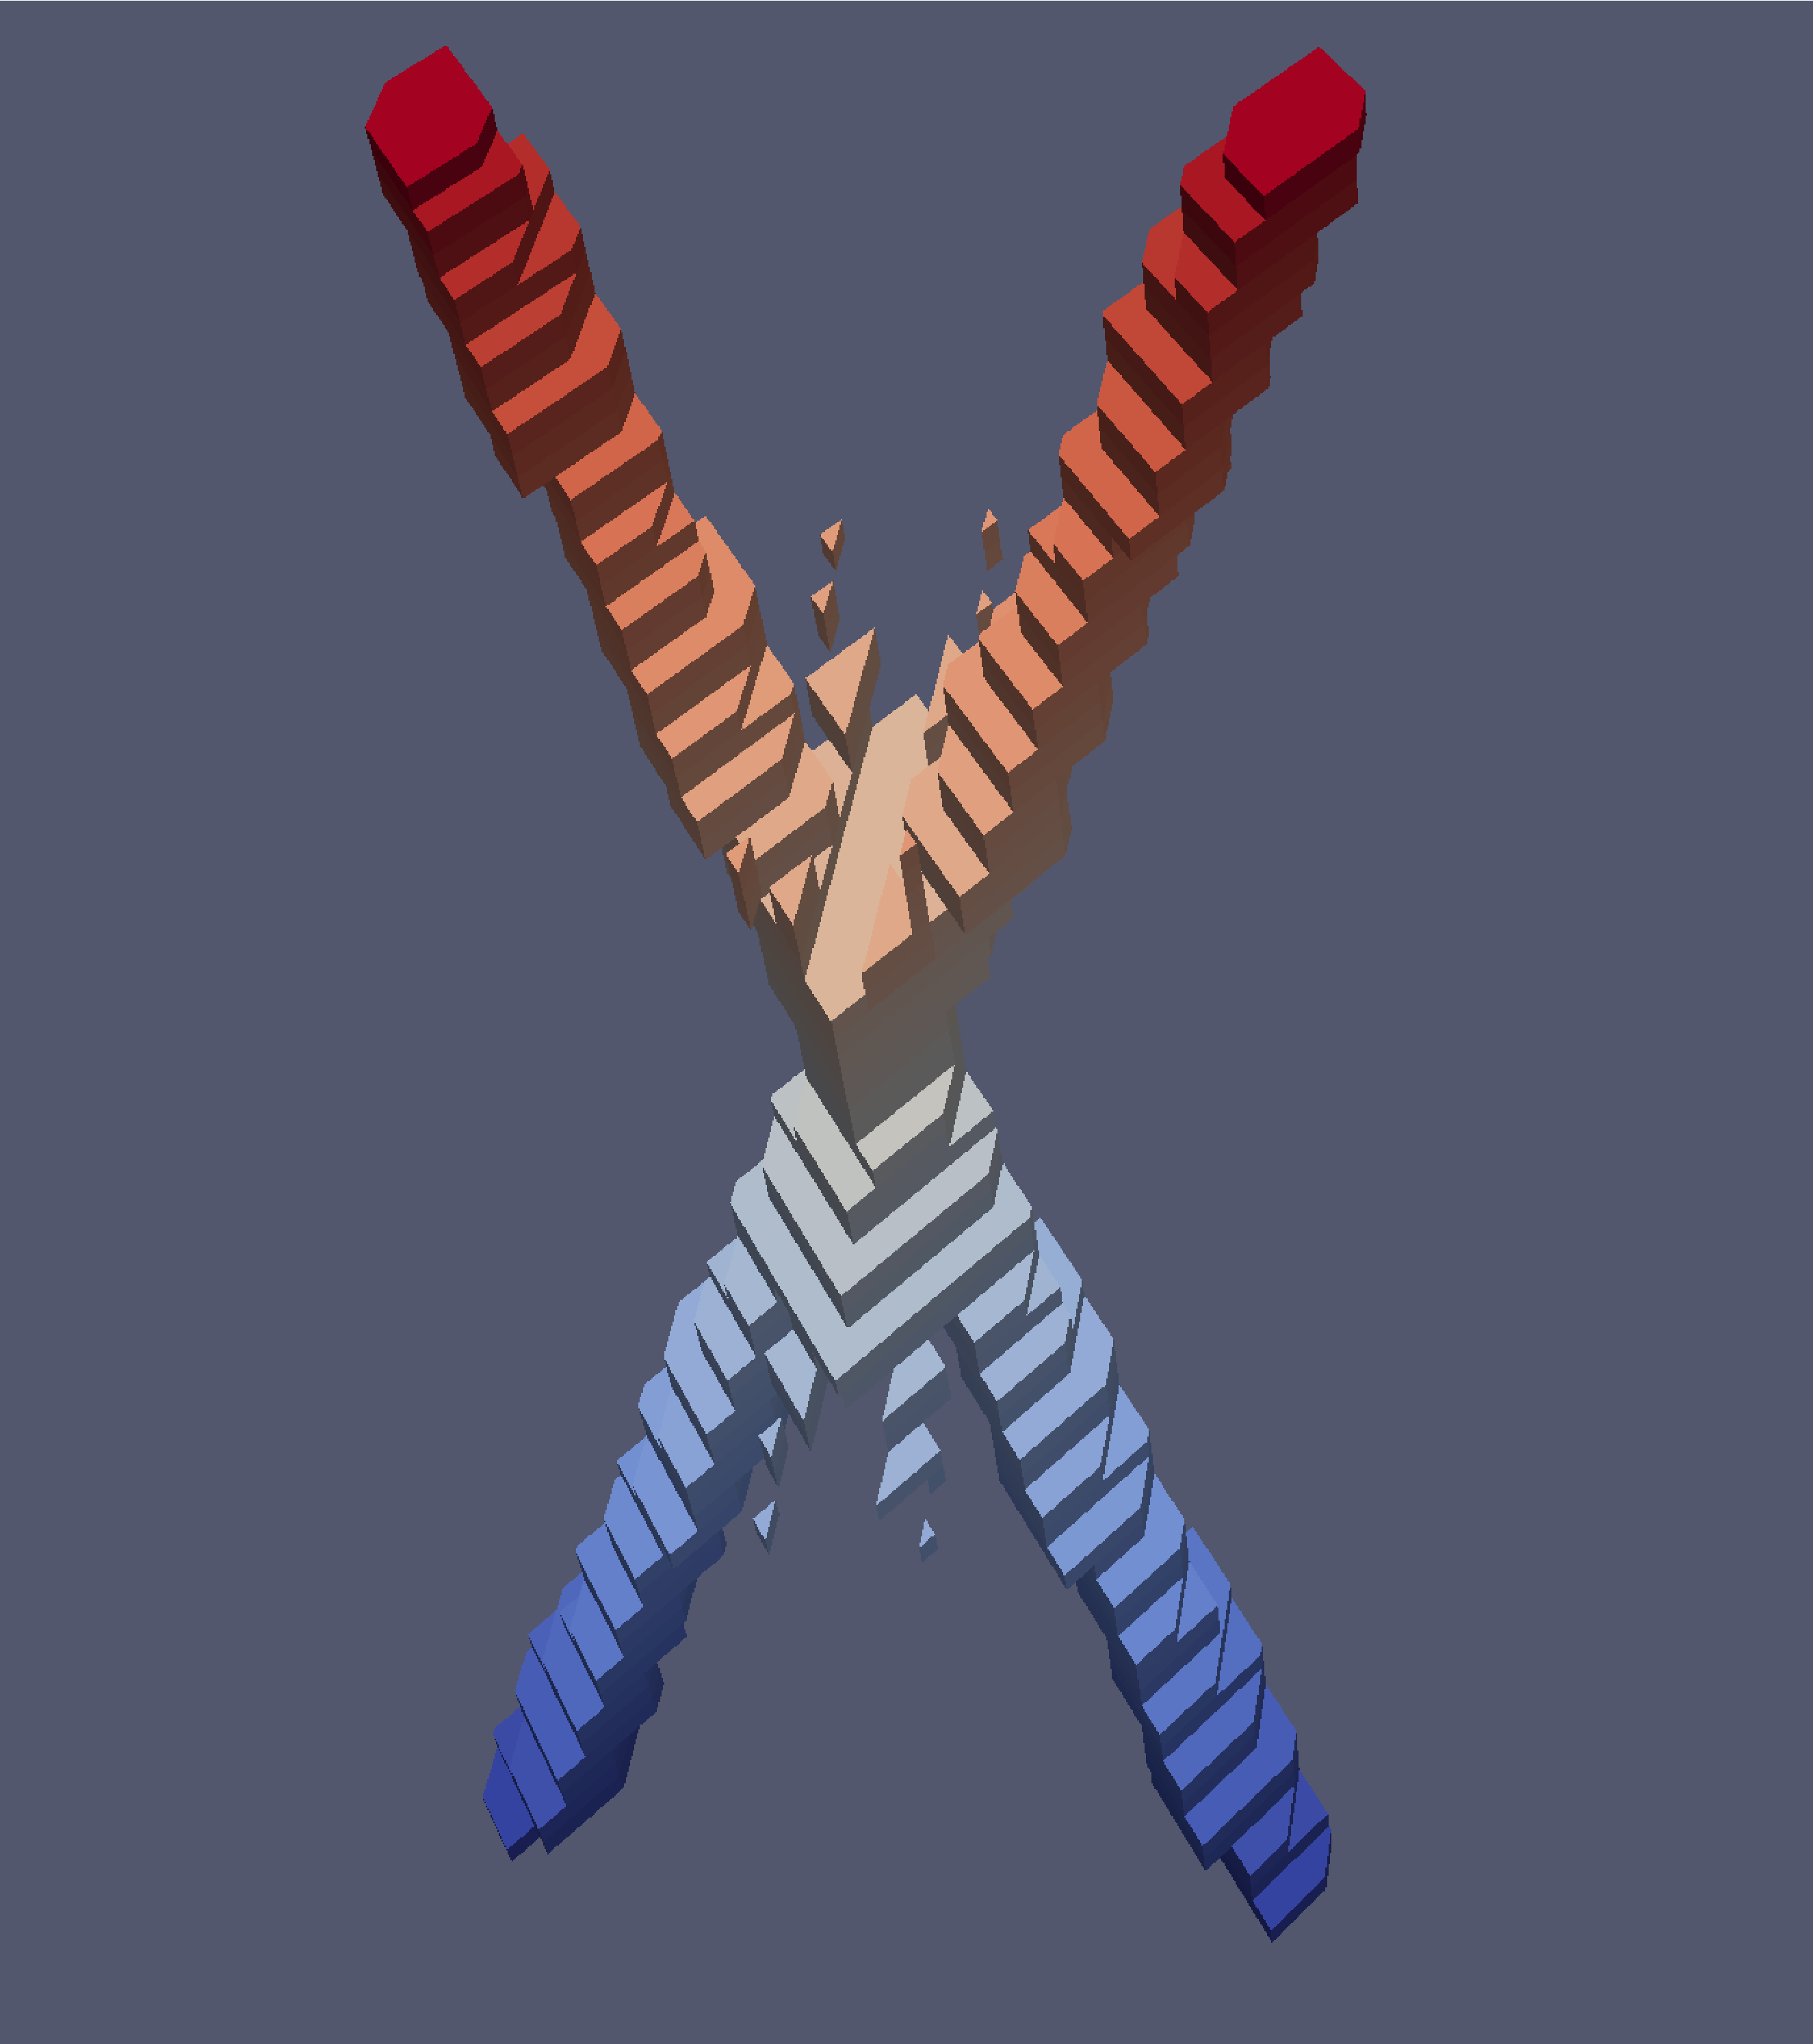
\includegraphics[width=\textwidth]{figs/grouping-threed.pdf}
\caption{\label{fig:grouping-threed}
The result of tiling a test pattern of two crossing ideal tracks.  Coloring simply indicates the slice number in which a blob resides.}
\end{figure}


\subsection{Solving}
\label{sec:Solving}

At this point, a solution may be attempted for $\vec{s}$, as defined in Section~\ref{sec:formalism}. 
The input to this step may be any graph of the form described in Section~\ref{sec:grouping}. 
The \texttt{b}-nodes of such a graph begin with zero associated ``value''. 
Solving is done by transforming a \textit{grouped graph} into the matrix equation~\ref{eq:solving}. 
The $\vec{m}$ vector is simply an ordered list of the values of the \texttt{m}-nodes. 
Their value is calculated by using their set of channels to look up the samples recorded in the associated \texttt{s}-node's slice. 
The initial $\vec{s_0}$ may be zero. 


\begin{figure}[htbp]
\centering
\includegraphics[width=\textwidth]{figs/solving-pipeline-example.pdf}
\caption{\label{fig:chain}
An illustrative example chain for solving.  Upstream a frame is narrowed to one APA and then sliced.  Each slice is sent to a per-face tiling which produce sets of blobs that are joined back into a per-slice set.  These blobs are clustered, grouped and finally ``solved''.  Subsequent solvers may be applied.  The results may finally be dispatched (not shown) as 3D space/charge points or projected back into 2D views depending on the needs of the application.}
\end{figure}

However as the output of solving also produces the same type of graph as its input a chain of solving steps may be constructed. 
In such a chain the $\vec{s}$ output of one solution may be transferred to an input starting $\vec{s_o}$ of the next as illustrated in figure~\ref{fig:chain}.  As hinted in this illustration, some parallel sub-pipelines may be defined.  The tiling is a per-face process and the entire chain shown is a per-APA process.  Downstream the cluster may be combined if the application is to study intra-APA activity.  A full WCT execution graph is shown in figure~\ref{fig:wctjob}.  This is one example.  Other configurations may slice the graph after the digitizer and replace the downstream subgraph with one that provides raw waveform data.  Or, the origin node which provides the ideal track energy depositions (\texttt{TrackDepos}) may be replaced with a richer source of depositions produced by Geant4 (eg, via LArSoft's \texttt{LArG4} module).

\begin{figure}[htbp]
\centering
\includegraphics[width=\textwidth]{figs/wct-sim-ideal-sn-nf-sp-img.pdf}
\caption{\label{fig:wctjob}
Graphical depiction of the Wire-Cell Toolkit simulation, signal processing, tiling and solving job for the six APA protoDUNE-SP.  Energy deposits enter on the left, fan-out to a per-APA pipeline.  Each pipeline applies field and electronics response to produce  induced signals.  Noise model is then applied and their sum is digitized.  The signal processing deconvolves the field and electronics response and the resulting reconstructed signals are sliced, tiled, clustered, grouped, solved and the final resulting clusters are dumped for plotting and evaluation.}
\end{figure}


Continuing on with the solving step, The matrix $R$ is simply the connection matrix of an induced subgraph formed by selecting only \texttt{(m-b)} edges.
The weight vector $\vec{\lambda}$ may is formed in an ad-hoc manner. 
An element of the vector starts with the magic number \texttt{9}. 
If it corresponding blob has an overlapping neighbor from a prior slice it is reduced by a magic factor of \texttt{3}. 
Likewise, if the subsequent slice at least one overlapping blob, another reduction of \texttt{3} is taken. 
Other weighting schemes may be investigated in the future.

The solving itself is performed by the RESS package and the elements of the resulting $\vec{s}$ solution vector are transferred back to a copy of the input graph, blob by blob.  The solution is graphically displayed as colors in figure~\ref{fig:solving}.

\begin{figure}[htbp]
\centering
\includegraphics[width=\textwidth]{figs/solved.pdf}
\caption{\label{fig:solving}
Solved blobs.  Colors indicate the amount of ionization electrons likely to be contained in any given blob region.  The pale gray indicates approximately one MIP, the rust/red color approximately two MIPs.  Most of the blue is above 10k electrons.}
\end{figure}

Thus, solving assigns a blob a (potentially) non-zero value which represents an estimation of the amount of ionization electrons that may be residing inside the blobs spatial extent. 
When successful, blobs with near zero value may be eliminated as being likely ``ghosts''. 
However, as shown in figure~\ref{fig:solving} some as ``ghost'' blobs are retained, their charge is lower than MIP level but nonzero and so thresholds must be applied carefully, if at all.

\begin{figure}[htbp]
\centering
\includegraphics[width=\textwidth]{figs/pdsp-data.pdf}
\caption{\label{fig:pdspdata}
A zoom in on a region of solved blobs from ProtoDUNE-SP data.}
\end{figure}

\begin{figure}[htbp]
\centering
\includegraphics[width=\textwidth]{figs/wcls-nf-sp-img.pdf}
\caption{\label{fig:pdspjob}
The WC/LS DFP graph for running NF+SP+IMG from inside art.}
\end{figure}


Figure~\ref{fig:pdspdata} shows a zoom in of reconstructed activity as solved blobs.  The job DFP graph is shown in figure~\ref{fig:pdspjob}.  Note that the per-APA pipelines are constructed by ``slicing'' the DFP graph in figure~\ref{fig:wctjob} in front of the SP components and attaching upstream NF and channel selector components.  The waveform input data is then taken from \texttt{art::Event}.  After SP, 2-way fanouts are used.  One port sends the per-APA frame into imaging and the other sends the same frame into a 6-way fanin so that the a full 6-APA frame can be merged and sent back to \texttt{art::Event} for saving as a vector of \texttt{recob:Wire} objects.




\end{document}